% tQRTguide.tex
% v1.2 released August 2014

\documentclass{tQRT2e}
\usepackage{fontspec}
\usepackage{subfigure}% Support for small, `sub' figures and tables
\usepackage{multirow}


\begin{document}

%\jvol{00} \jnum{00} \jyear{2014} \jmonth{August}

% \articletype{GUIDE}% NOT NEEDED FOR A RESEARCH ARTICLE IN THIS JOURNAL%

\title{Detection of Insulation Flaws and Thermal Bridges in Insulated Truck Box Panels}

\author{Lei, Lei$^{\rm a}$$^{\ast}$\thanks{$^\ast$Corresponding author. Email: lei.lei.1@ulaval.ca
\vspace{6pt}},  Alessandro Bortolin$^{\rm b}$, Paolo Bison$^{\rm b}$ and Xavier Maldague$^{\rm a}$\\\vspace{6pt}  $^{a}${\em{Computer Vision and Systems Laboratory, University Laval, Quebec, Canada}};
$^{b}${\em{CNR-ITC Padova, Italy}} \\\received{}}

\maketitle

\begin{abstract}
This paper focuses on the detection of defects and thermal bridges in insulated truck box panels, utilizing infrared thermography. Unlike the traditional way in which passive thermography is applied, this research uses both heating and cooling methods in active thermography configurations. Lamp heating is used as the hot external stimulation, while a compressed air jet is applied as the cold external stimulation. A thermal camera captures the whole process. In addition, numerical simulations under COMSOL$^®$ platform are also conducted. Experimental and simulation results for two situations are compared and discussed.

\begin{keywords}infrared thermography; liquid nitrogen cooling; comsol; truck panel; thermal bridge
\end{keywords}

\end{abstract}


\section{Introduction}

The increasing cost of energy has made energy saving a vital necessity in the current world. One of the examples involves, “Maintaining the cold chain”: the correct transport of perishable foodstuffs in refrigerated vehicles, especially for dairy products, meat and frozen foods, which has become the key part of every successful distributor’s food safety program. Therefore, a suitable thermal insulation implemented in refrigerated vehicles is essential for saving energy while maintaining an appropriate conservation of the foodstuffs. There are some agreements concerning thermal insulation tests which ensures the suitability for the transport of food in refrigerated conditions, for example ATP: “The Agreement on the Transport of Perishable foodstuffs” \cite{Geneva1970}, which establishes standards for the international transport of perishable food between the states that ratify the treaty since 1970.

The Construction Technologies Institute of the Italian National Research Council (ITC- CNR), our collaborator, hosts a wide testing facility for refrigerated vehicles or insulated roll containers and it is also authorized by the Italian Ministry of Transport to perform such ATP tests \cite{Tassou2009,dragano2009experimental}. The ATP standard test is a procedure that measures the insulating performance of truck panels with a global approach; however, if there are some local flaws or thermal bridges inside the panels, which could not be measured by ATP tests, then the insulation and the stability of the temperature can no longer be guaranteed. Usually truck panels are manufactured from composite insulated materials in order to ensure that the interior of the truck is maintained at a cold temperature \cite{Bortolin2015}. Therefore, this research attempts to detect the local flaws inside a truck panel specimen with a straightforward visualization.


\section{Samples \& Methods}

\begin{figure}
	%\begin{center}
	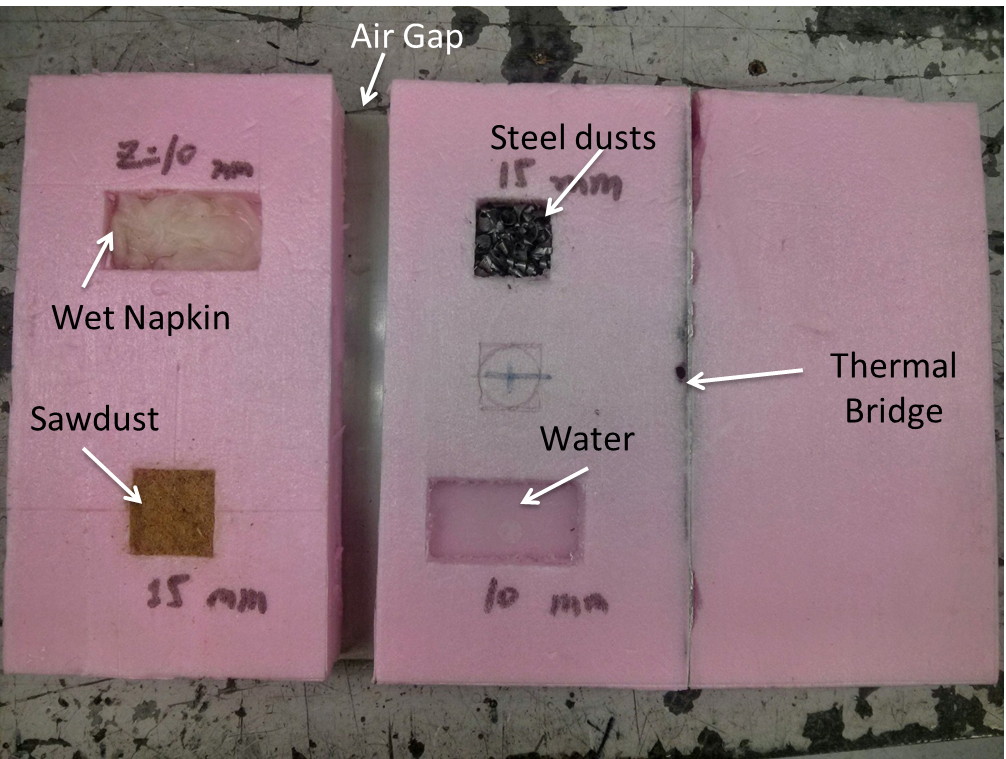
\includegraphics[width=7.33cm, height=5.5cm]{Panel_detail}
	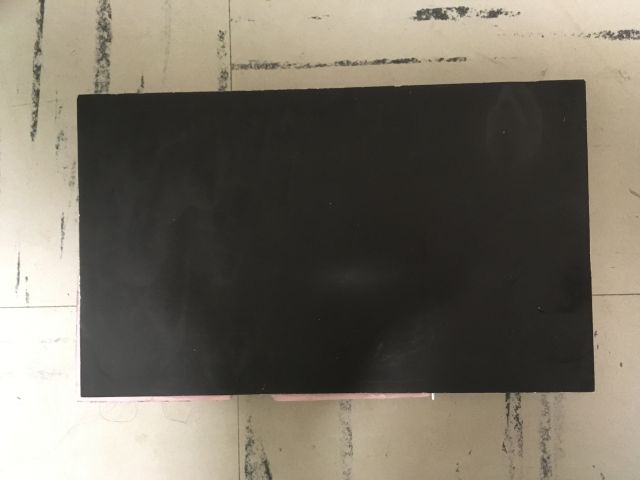
\includegraphics[width=7.33cm, height=5.5cm]{Panel_done}
	\caption{Details of defects inside the specimen (left) and final specimen to test (right) }
	\label{panel}
	%\end{center}
\end{figure}
\indent \indent In this research, several possible different types of defects inside a truck panel will be examined.  A panel containing these defects has been constructed and is shown in Figure~\ref{panel}. The insulated material used is polystyrene, inserted between two thin aluminum plaques. A small aluminum plaque is embedded ‘vertically’ inside acting as a thermal bridge. Other flaws are defined as an air gap, a defect involving a wet napkin, a hole filled with sawdust, another hole filled with steel dust and a defect filled with water; these are representative of current truck box fabrication and potential defects. The simulated panel was painted before the test to increase emissivity of aluminum. Particularly the thermal bridge and the defect of water are the main targets to identify, since they appear regularly in the gaps of truck panels. A sound area with no defects has also been defined for later comparison and reference, which is located at the center of the specimen. The specification details can be found in Table~\ref{Tab_spe}.
\begin{table}
	\centering

	\caption{Specimen specification details.}
	\begin{tabular}{c|c|c|c|c}
		\hline
		& \textbf{Aluminum,plaques} & \textbf{Foam}       & \textbf{Air Gap}     & \textbf{Thermal Bridge} \\ \cline{2-5} 
		\multirow{2}{*}{Dimensions (mm)} & 250*150*1        & 250*150*25 & 15*150 *25  & 1*150*25       \\ \cline{2-5} 
		& \textbf{Wet Napkin}       & \textbf{Sawdust}    & \textbf{Steel dusts} & \textbf{Water}          \\ \cline{2-5} 
		& 40*20*10         & 20*20*15   & 20*20*15    & 40*20*10       \\ \hline
	\end{tabular}
	\label{Tab_spe}
\end{table}
%\begin{table}
%	\centering
%\tbl{Specimen specification details.}
%\begin{tabular}{lcccc}
%	\toprule
%	\multirow{4}{*}{\centering Dimensions (mm)}&
%	 Aluminum plaques & Foam & Air Gap & Thermal Bridge \\ 
%	 250*150*1 & 250*150*25 & 15*150*25 & 1*150*25 \\ 
%	 Wet Napkin & Sawdust & Steel dusts & Water \\ 
%	40*20*10 & 20*20*15 & 20*20*15 & 40*20*10 \\ 
%	\botrule 
%\end{tabular}
%\label{Tab_spe}
%\end{table} 
% \begin{table}
% \tbl{Specimen specification details.}
% {\begin{tabular}[l]{@{}lcccccc}\toprule
%   Class$^{\rm a}$ & $\gamma _1$ & $\gamma _2$$^{\rm b}$
%          & $\langle \gamma \rangle$
%          & $G$ & $|{\bm f}|$ & $\theta _{c}$ \\
% \colrule
%   BL Lacs & 5 & 36 & 7 & $-4.0$ & $1.0\times 10^{-2}$ & 10$^\circ$ \\
%   FSRQs & 5 & 40 & 11 & $-2.3$ & $0.5\times 10^{-2}$ & 14$^\circ$ \\
% \botrule
% \end{tabular}}
% \tabnote{$^{\rm a}$This footnote shows what footnote symbols to use.}
% \tabnote{$^{\rm b}$This footnote shows the text turning over when a long footnote is added.}
% \label{sample-table}
% \end{table}

In order to localize the possible defects inside the specimen, active infrared thermography \cite{Maldague2001theory,Balageas2016}, one of the non-destructive testing \& evaluation techniques, is applied for diagnostics. Basically, the specimen to inspect is thermally stimulated and the subsequent temperature evolution is recorded to reveal possible subsurface flaws. In this study two opposing approaches of external stimulations are then applied with the goal of clearly detecting the flaws in the truck panel. One approach uses a traditional lamp heating; the other method involves air cooling. 


% \section{Additional features}
\section{Experimental set-up}
The experiment is set up with the following equipment, shown in Figure~\ref{Exp}:
\begin{figure}
	\centering
	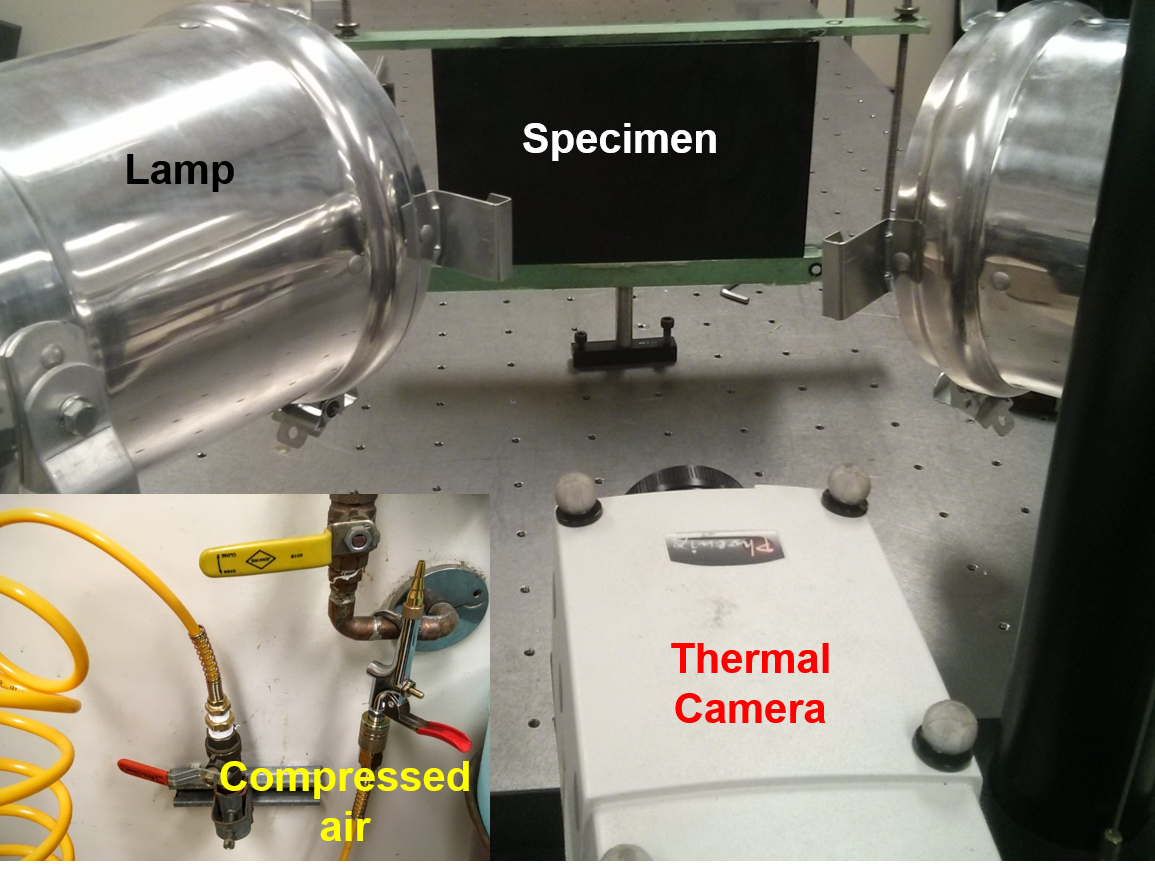
\includegraphics[scale=0.5]{Exp}
	\caption{Experimental set-up}
	\label{Exp}
\end{figure}

\begin{itemize}
  \item Two halogen lamps with a total heat source of 1000 $W$;
  \item A FLIR Phoenix thermal camera (640×512 pixels, InSb, 3-5 $\mu m$);
  \item Compressed air connected by a tube and a nozzle with a diameter of 5 $mm$ (zoomed bottom left).
\end{itemize}

The whole procedure of study is described as follows:  

For lamp heating, two halogen lamps are employed at a distance of 0.4 $ m $ and at an angle of about 45° for the purpose of homogeneously heating the surface. The duration of the heating process is only 20 $ s $.   

For air cooling, compressed air with a temperature of about 15° (details are shown in Table~\ref{air_cool}) is sprayed at a distance of 0.4 $m$ and at an angle of about 45° in the \textbf{left} front of the specimen’s surface. It is a central spray form left to right along the specimen surface. By doing this, one tries to avoid the direct squirt on the area of defects. In this process, contrary to the heating one, the specimen was preheated to about 30$ °C $, which is similar to the real situation for detection of truck panel defects in the summer. The duration of the cooling-down process is about 20 $ s $ as well.   
 \begin{table}
 \tbl{Air-Cooling parameters.}
 {\begin{tabular}[l]{@{}cccccc}\toprule
   \textbf{Material} & \textbf{Outlet Pressure} & \textbf{Flow}
          & \textbf{Nozzle diameter}
          & \textbf{Density} & \textbf{Temperature} \\
 \colrule
   Compressed Air & 6 bar & 0.0224 $m^3/s$ & 6.35 $mm$ & 1.2041 $kg/m^3$ & 15° \\
 \botrule
 \end{tabular}}
% \tabnote{$^{\rm a}$This footnote shows what footnote symbols to use.}
% \tabnote{$^{\rm b}$This footnote shows the text turning over when a long footnote is added.}
 \label{air_cool}
 \end{table}
Both processes have been recorded by the thermal camera with a resolution of 640$\times$512 pixels.  

\section{Simulation models}
To obtain a comparative result, numerical models have also been developed, with the finite element method under COMSOL Multiphysics$^{®}$. In addition to the similar transient problem appearing in experimental conditions, static regime simulation is also taken into account. The influences of heat conduction, convection and radiation (surface-to-surface and surface to ambient) on the heat flow through the defect have been simulated and analyzed.

The physical nature of the heat transfer is governed by the differential equations such as the one of the heat transfer by conduction, convection and radiation with temperature dependent thermal properties of materials involved. The differential equation, governing pure conductive heat transfer, to be solved on the model domain is: 

\begin{equation}
\rho C_p \frac{\partial T}{\partial t}-\nabla \cdot (k\nabla T) = 0
\end{equation}
where $\rho$ is the density (\textit{$kg/m^3$}),   $C_p$ is the material heat capacity at constant pressure ($J/(kg·K)$), $ T $ is absolute temperature ($K$) and \textit{k} is the material thermal conductivity ($W/(m·K)$) and $ t $ is the time (s).

The boundary condition included heat transfer by convection and radiation from the object surfaces and the  heat  source $q_0$  applied on the front surface as the following: 
\begin{equation}
n(k\nabla T) = q_0 + h_{cv}(T_{amb}-T)+\sigma \epsilon(T_{amb}^4-T^4)
\label{eqf}
\end{equation}
where $n$ is the normal direction of surface, $ h_{cv} $ is the constant convective heat transfer coefficient, $\sigma$ is the Stefan-Boltzmann constant  and $\epsilon$ is the emissivity that is the ratio of radiant emittance of an object to that of a blackbody at the same temperature. Its value lies from zero for a non radiating object and 1.0 for a blackbody. $ T_{amb} $ is the room temperature.

\begin{figure}[ht]
	%\centering
    \hspace{-8pt}
    \subfigure[Heating with two halogen lamps]
    {
        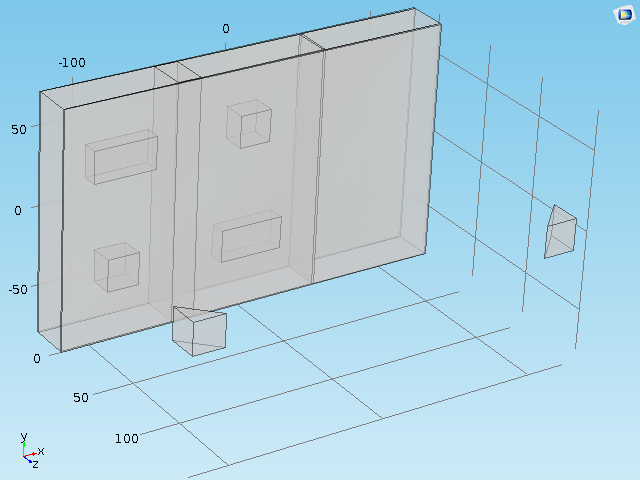
\includegraphics[width=7.33cm, height=5.5cm]{Flash_model2}
    }
    \hspace{-5pt}
    \subfigure[Cooling with compressed air by a nozzle ]
    {
        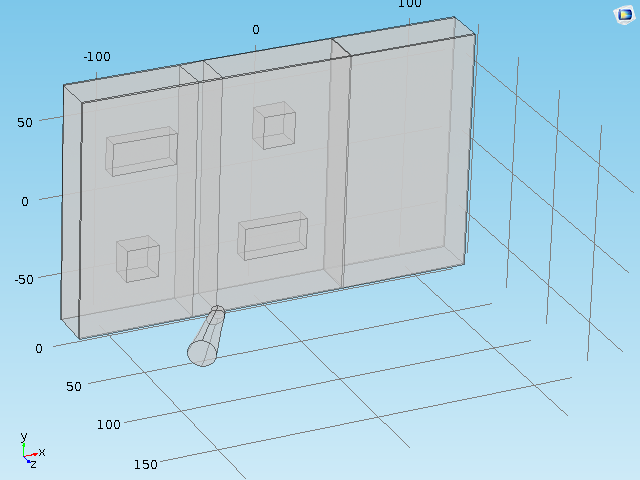
\includegraphics[width=7.33cm, height=5.5cm]{Laminar_model2} 
    }
	\caption{Simulation 3D models transparency view}
	\label{models}
	%\end{center}
\end{figure}
Parameters for each model are introduced as follows:\\
For lamp heating, heat transfer in solid with surface-to-surface radiation module is applied in the model. Therefore, one assumes that there is no effect by convective transfer [$h_{cv}=0$ in eq. \ref{eqf}]

For air cooling, heat transfer and single phase laminar flow modules are implemented since the convection effect in this case has a more significant influence. the multiphysics setting is also set as a non-isothermal flow. Then one assumes that there is no effect by the heat source [$ q_0=0 $ in eq. \ref{eqf}]

For the static regime, a simple heat transfer in solid module is employed. Thus one has $ h_{cv} $=0 and $ q_0=0 $ in eq. \ref{eqf}

All materials properties applied in the models can be found in Table~\ref{mat_pro}. 
 \begin{table}[ht]
  	\centering
  	\scriptsize
 	\caption{Materials properties.}
% \tbl{Materials properties.}
 {\begin{tabular}{p{1.5cm}|p{1.5cm}p{1.5cm}p{1.5cm}p{1.5cm}p{1.5cm}p{1.5cm}}
 	\hline
	      & Density $\rho [Kg/m^3] $
	      & Thermal conductivity  $k [W/(m\cdot K)] $
          & Heat Capacity $C_p [J/(Kg\cdot K)]$
          & Surface Emissivity $\epsilon$
          & Dynamic viscosity $\mu [10^{-5}kg/m\cdot s]$ 
          & Ratio of specific heat $\gamma$   \\
	 \hline
   Aluminum (plaques and thermal bridge)	&2700	&238	&900 &0.77 & & \\
   Foam	&24	&0.03	&1300 & & & \\
   Air	&1.2 &0.024	&1.005 & &1.846 &1.4 \\
   Sawdust	&192	&0.08	&900 & & & \\
   Water &1000	&0.58	&4.18 & & &1.33 \\
   Steel &7850	&44.5	&475 & & & \\
   Lamps &8700	&400	&10 &0.99 & & \\
	 \hline
 \end{tabular}}
% \tabnote{$^{\rm a}$This footnote shows what footnote symbols to use.}
% \tabnote{$^{\rm b}$This footnote shows the text turning over when a long footnote is added.}
 \label{mat_pro}
 \end{table}


\section{Results and Discussion}
Several image post-processing methods can be applied, such as Pulsed Phase Thermography (PPT)\cite{Maldague1996}, Principal Component Thermography (PCT)\cite{Rajic2002}. PCT technique uses “singular value decomposition (SVD) to reduce the matrix of observations to a highly compact statistical representation of the spatial and temporal variations relating to contrast information associated with underlying structural flaws”. Temperature distributions of the panel surface for both cases are presented in Figure~\ref{exp_res} and Figure~\ref{sim_res} (front View). Both lamp-heating and air-cooling images shown are the third image post-processed by the PCT technique. It is clear that in experimental results, the defects of metal and water are easy to identify, in both heating and cooling cases. The thermal bridges are slightly clearer in the cooling process than the heating process. However, the defect of the wet napkin has almost not been displayed in both cases. On the other hand, in simulation results, due to the ideal conditions, one can clearly notice the four defects mentioned above. Figure 5 indicates that there is a more obvious view of defects in lamp heating as opposed to air cooling, the detection time of the latter is much less.
\begin{figure}
%	\begin{center}
    %\centering
    \hspace{-20pt}
    \subfigure[lamp heating raw image]
    {
        \includegraphics[scale=0.54]{Raw_heating.png}    
    }
    \hspace{-10pt}
    \subfigure[air cooling raw image]
    {
        \includegraphics[scale=0.54]{Raw_cooling.png}
    }\\

    \hspace{-20pt}
    \subfigure[PCT 3$^{rd}$ image of lamp heating]
    {
        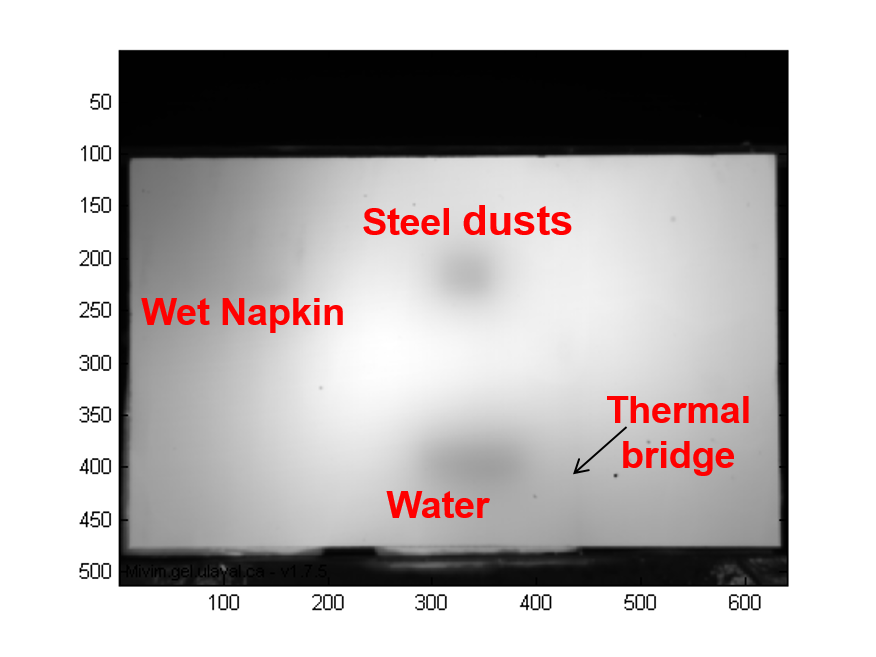
\includegraphics[scale=0.54]{Heat_FT_AMP}
    }   
    \hspace{-10pt}
    \subfigure[PCT 3$^{rd}$ image of air cooling]
    {
        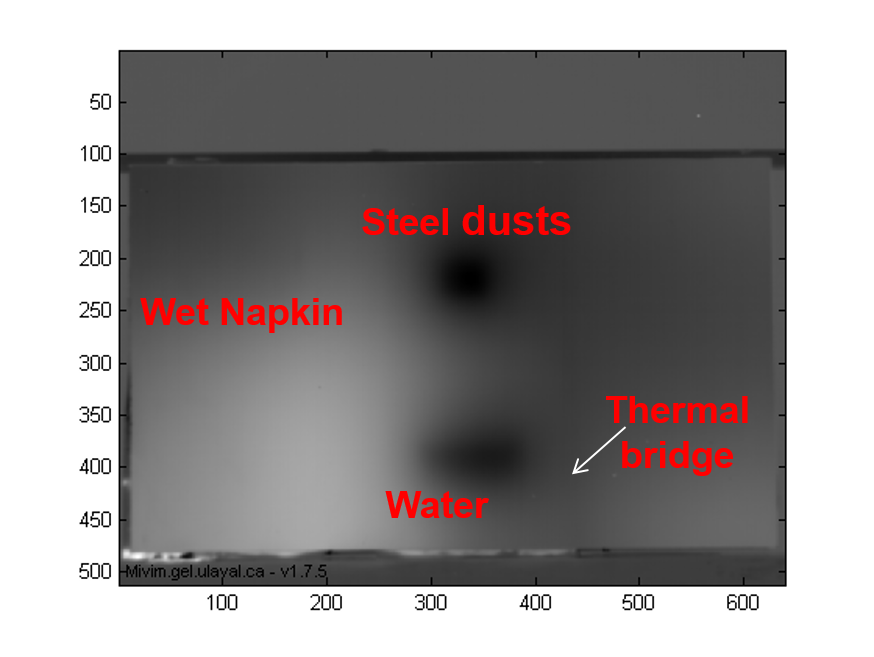
\includegraphics[scale=0.54]{Cool_PCT3_2}
    }
	\caption{Experimental results}
	\label{exp_res}
%	\end{center}
\end{figure}

\begin{figure}
%	\begin{center}
    %\centering
    \hspace{-20pt}
    \subfigure[temperature distribution of lamp heating results]
    {
       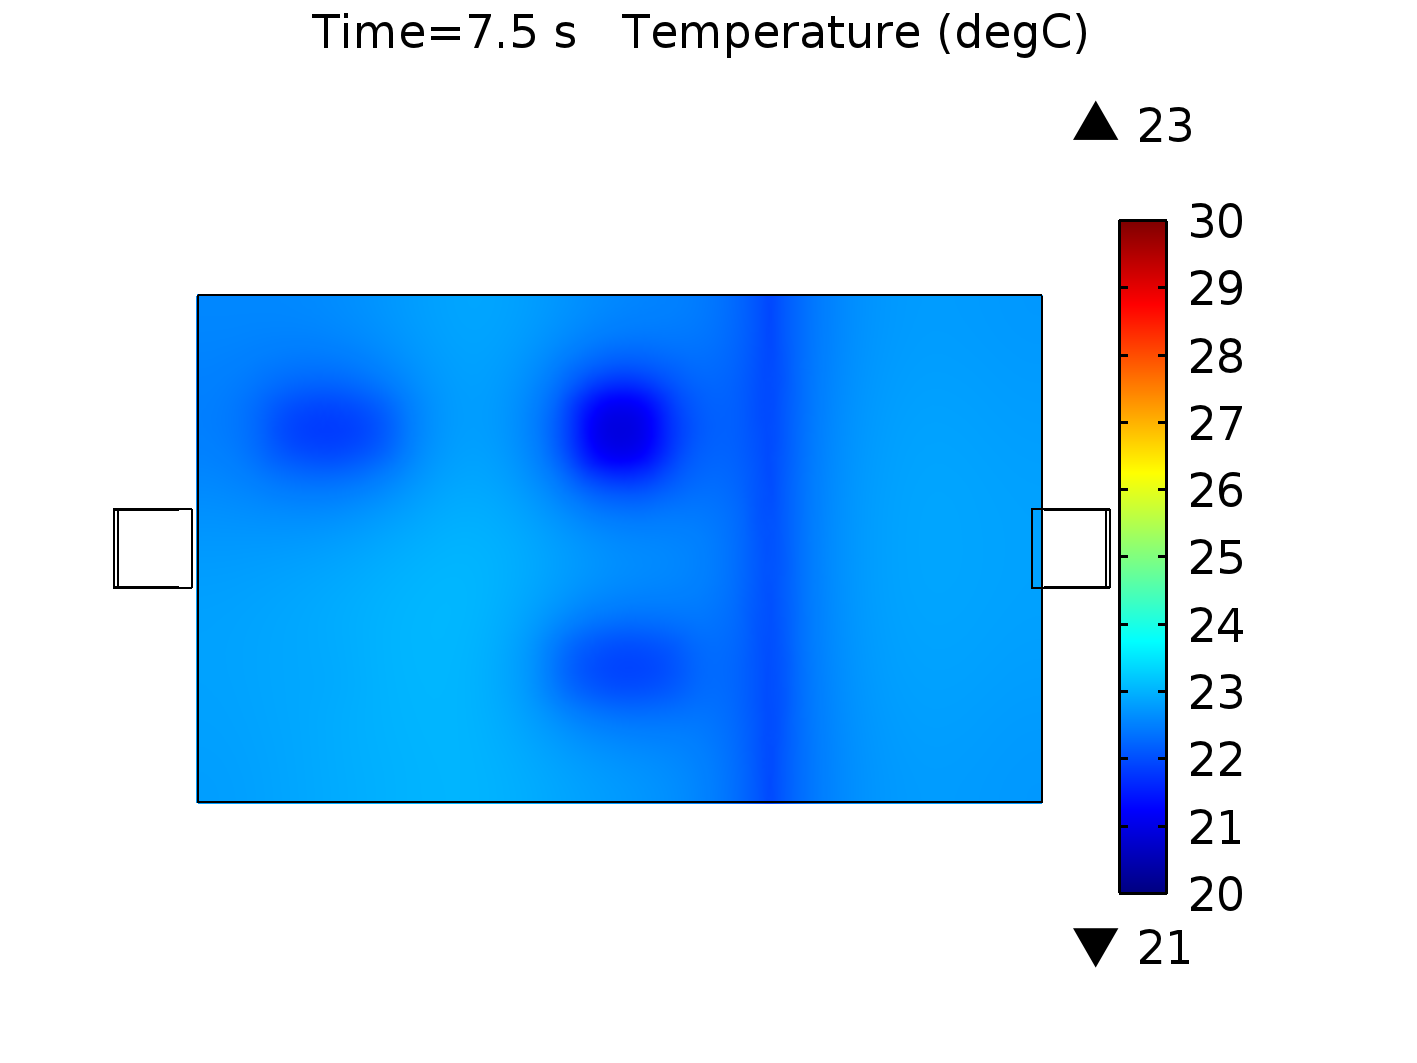
\includegraphics[scale=0.7]{Truck_panel_flash_03}
    }
    \hspace{-5pt}
	\subfigure[temperature distribution of air cooling results]
    {
        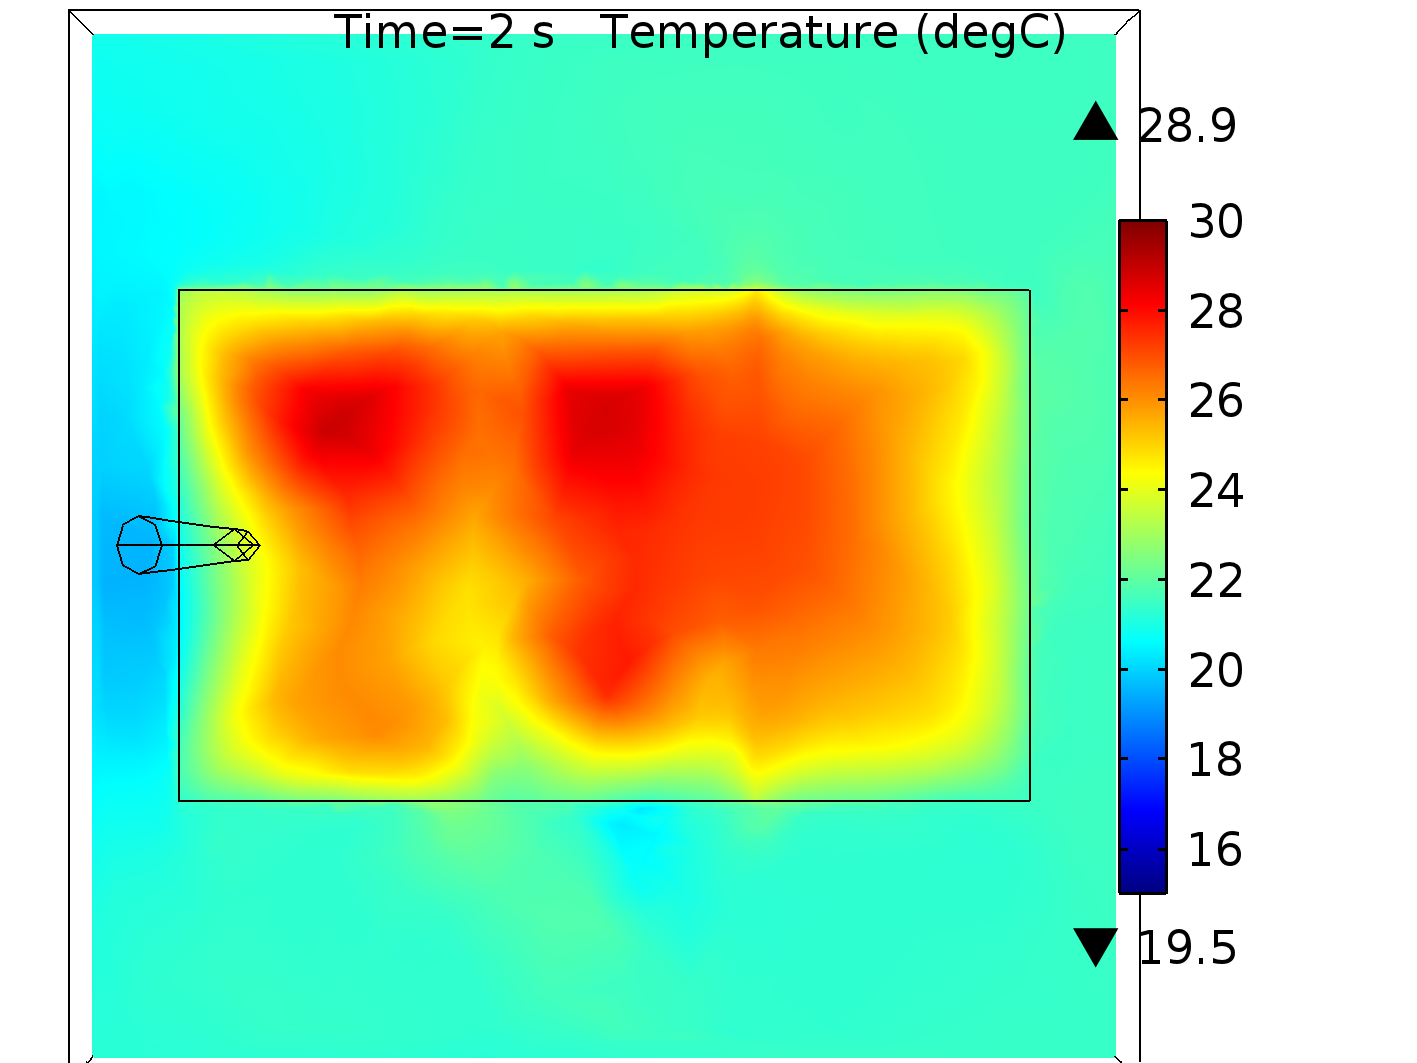
\includegraphics[scale=0.7]{Truck_panel_laminar_final_7_3}
    }
	\caption{Simulation results}
	\label{sim_res}
%	\end{center}
\end{figure}
Nonetheless, in both experiments and simulation models the sawdust defect was impossible to detect, due to its thermal conductivity close to polystyrene. The same situation occurred for the air gap, which could not be detected, neither.  

From the observations above, a discussion of detectability of defects can be summarized as:
In comparison, both methods can only detect four defects rather than all. Although the halogen lamps were positioned to achieve a high energy pulse and a homogeneous heating as well, there is still an inhomogeneous distribution of temperature with a maximum in the middle of the sample and smaller values at the edges and especially in the area of wet napkin and sawdust (left edge part in the image). This might explain that wet napkin was displayed in computational results (ideal condition) while one could not detect it in real heating process. 

For air cooling, the jet impingement can not be neglected. Since it was not a uniform spray to the sample surface, the squirt was produced in left center along the surface of the specimen to the right. Therefore, the areas of wet napkin and sawdust were not cooled well. The main part of air jet was deployed on the steel dust, water and thermal bridge defects zones. This might explain that in simulation model (ideal condition), at the first beginning of the cooling process the four defects appeared and in experimental test one could not observe the wet napkin defect.

In addition to the straight views comparison in the thermal images, the quantitative computation has also been carried out at the same time. Temperature evolutions in time for both cases are illustrated in Figure~\ref{exp_fig} and Figure~\ref{sim_fig}. Here one calculates the cases of the water and thermal bridge (which are generally found in truck panels) compared to the sound area without defects. In both situations, experimental and simulation, it is observed that during lamp-heating, the temperatures of the thermal bridge and water defect area increased more slowly than the sound area value, while they decreased more slowly as well during air cooling. Quantitatively, for lamp heating, all defect temperature areas are lower than the sound area temperature. For air-cooling, on the contrary, all temperatures of defect areas are higher than that of the sound area (the descendant curve at the end of heating profile is due to the delay between the camera and lamps).  
\begin{figure}
	%	\begin{center}
    %\centering
    \hspace{-20pt}
    \subfigure[temperature evolution by lamp heating]
    {
        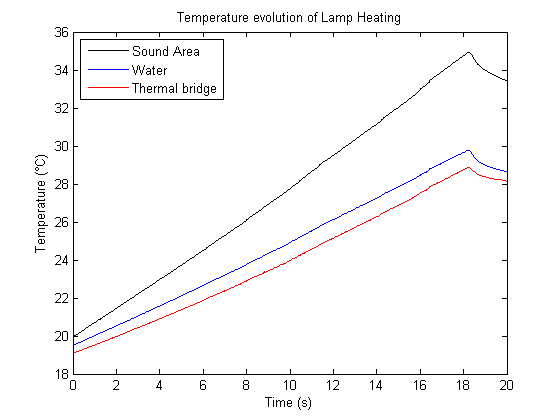
\includegraphics[scale=0.55]{heating_evolution5}    
    }
    \hspace{-12pt}
    \subfigure[temperature evolution by air cooling]
    {
        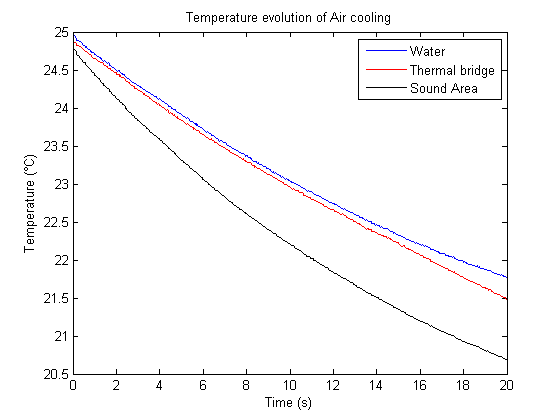
\includegraphics[scale=0.55]{cooling_evolution4}    
    }
	\caption{Experimental quantitative results of panel surface}
	\label{exp_fig}
	%	\end{center}
\end{figure}

\begin{figure}
	%	\begin{center}
    %\centering
    \hspace{-18pt}
    \subfigure[temperature evolution by lamp heating]
    {
        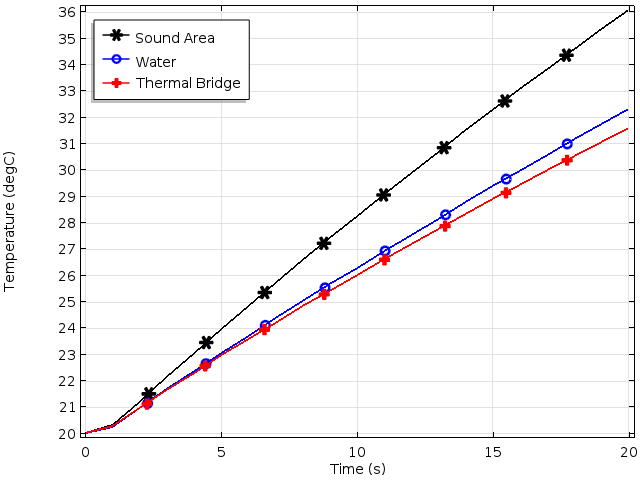
\includegraphics[scale=0.46]{Truck_panel_Flash_TGraph_4}    
    }
    \hspace{6pt}
    \subfigure[temperature evolution by air cooling]
    {
        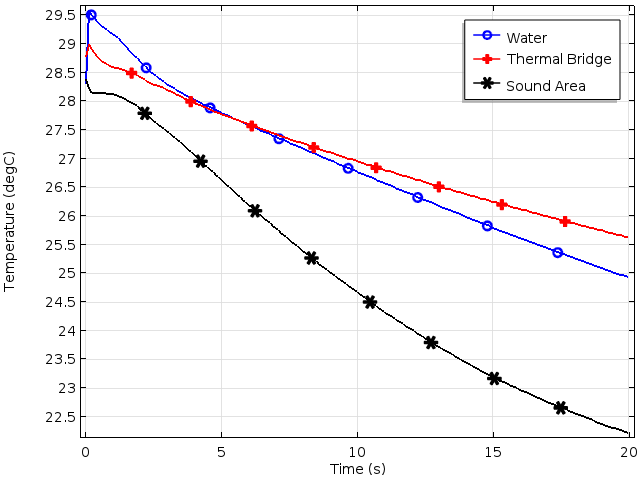
\includegraphics[scale=0.46]{Truck_panel_laminar_TGraph_4}
    }
	\caption{Computational quantitative results of panel surface}
	\label{sim_fig}
	%	\end{center}
\end{figure}
From the results above, one calculates the thermal contrasts between two defects and the sound area. Moreover, the corresponding contrast peaks have been determined, shown in Table~\ref{tab_TCP}.
\begin{table}[ht]
	\centering
	\caption{Thermal contrast peak table ($˚C$)}
	\begin{tabular}{l|cc|cc}
		\hline
		& \multicolumn{2}{c|}{Experiment} & \multicolumn{2}{c}{Simulation} \\
		 & Heating & Cooling & Heating & Cooling \\
		\hline
		Sound Area & 0 & 0 & 0 & 0 \\
		Water & 5.17 & 1.08 & 3.80 & 1.6 \\
		Thermal bridge & 6.07 & 0.87 & 4.52 & 2.3 \\  
		\hline
	\end{tabular}
	\label{tab_TCP}
\end{table}
This table indicates that for both cases, the lamp heating method has a higher contrast peak than the air cooling method. While comparing the temperature evolution profiles, the air cooling method requires less time to reach the contrast peak. This coincides with the detection of flaws in thermal images view.

For further exploration of the detection of each method, one defines here a “threshold” with $C_p$ = 1 as the limit of detection, where $C_p$ is the peak of thermal contrast. As the experimental and computational results are very comparable from above, we change the size (diameter) of the water defect and the thickness of thermal bridge in both heating and cooling models to seek the limit of detection. For supplementary comparison, we add also a regular situation: the static regime. This acts as the traditional passive thermography. One imagines that the truck is under sunshine in the exterior during summer, and inside temperature is kept as the cold chain, which could be -20°C. Then a thermal camera from outside observes the truck panel. Different sizes of water defects and widths of the thermal bridge have been performed during the same period (20 $s$) for this case.

All the computational results are presented in the following figures (Figure~\ref{sim_fig_stat} and Figure~\ref{sim_fig_ht})
\begin{figure}
	%	\begin{center}
    \hspace{-15pt}
    \subfigure[Evolution of static regime]
    {
        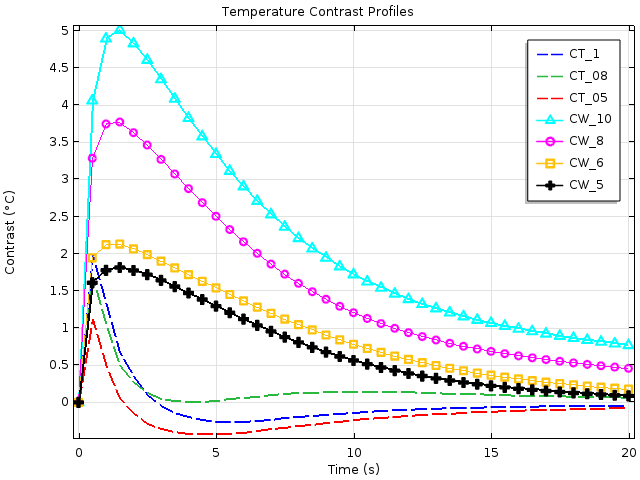
\includegraphics[scale=0.46]{Truck_panel_Model_Static_Contrast}    
    }
    \subfigure[Evolution of air cooling]
    {
        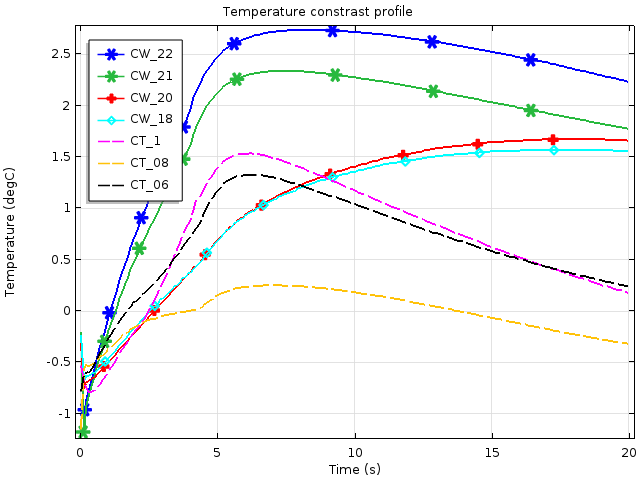
\includegraphics[scale=0.46]{Truck_panel_Model_laminar}
    }
	\caption{Temperature contrast profiles of simulation models}
	\label{sim_fig_stat}
	%	\end{center}
\end{figure}

\begin{figure}
	%	\begin{center}
	\hspace{-15pt}
    \subfigure[Evolution of thermal bridge]
    {
    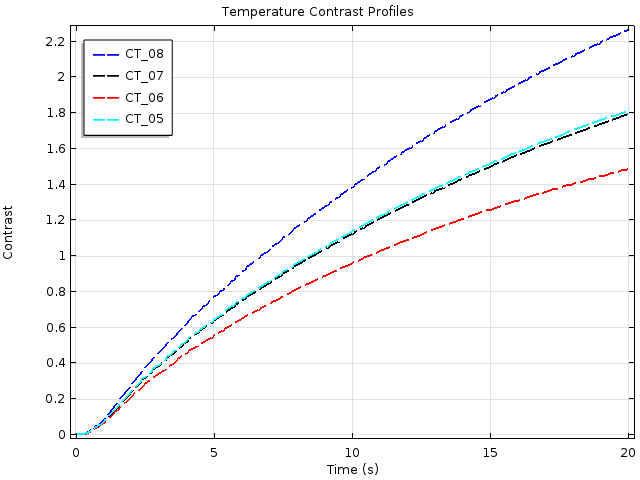
\includegraphics[scale=0.46]{Truck_panel_Model_Flash_CT}    
    }
    \subfigure[Evolution of water defects]
    {
    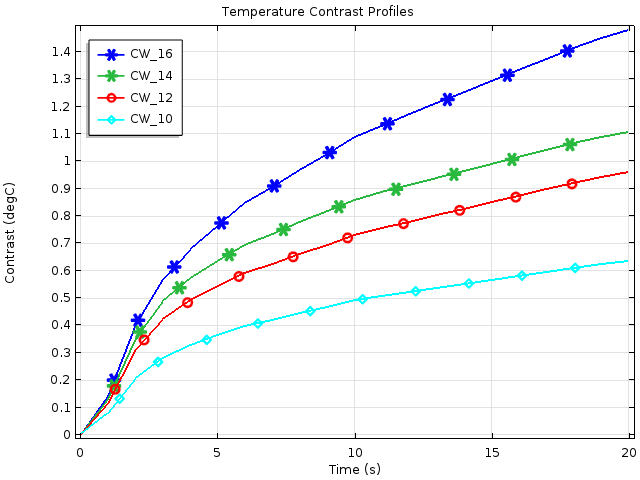
\includegraphics[scale=0.46]{Truck_panel_Model_Flash_CW}    
    }
	\caption{Temperature contrast profiles of Lamp heating model}
	\label{sim_fig_ht}
	%	\end{center}
\end{figure}
Where $ CT $ represents the contrast of the thermal bridge, $ CW $ represents the contrast of the water defect in all figures, and the numbers indicate the diameter and the thickness respectively. 

From the results above, it is evident that the static regime and lamp heating have more consistent profiles for the two types of flaws. All profiles in static regime increased rapidly at the beginning, as a consequence of temperature difference between sound area and defects area. Soon they all reached at a peak value subsequently. The contrast peak values varied according to different sizes of defect. Evidently, the contrast values of water defects are more sizable than that of thermal bridge. Then all profiles decreased gradually since the propagation of the heat inside the panel. In the end, they tend around whole uniform. 

While in air-cooling case there are several non-uniform profiles, nonetheless, the contrast profiles of water defect with large sizes (21 $mm $ and 22 $ mm $) and those of thermal bridge with all sizes have the similar tendency. They increased at the beginning due to the convection by air and then decreased slowly because of the propagation of heat dissipation inside the panel. However, for the contrast profiles of water defects with smaller sizes (20 $ mm $ and 18 $ mm $), they appeared as a unique increase. They might decrease again for long time modeling. An unusual thing found in air-cooling model was the thermal bridge with 0.8 $ mm $ thick had a lower contrast than those of 1 $mm $ and 0.6 $ mm $, this might be due to the influence of disturbance by airflow. 

For lamp-heating situation, one can observe that whole contrast profiles had a uniform tendency, which they all raised with time. This is as a result by radiation heating.

Finally, according to our “threshold” $ C_p  = 1$, then from the figures the limit of detection of these three cases is (during a period of time [20 $s$]): 
\begin{itemize}
  \item static regime: water defect diameter 5 $ mm $; thermal bridge thickness 0.5 $ mm $.
  \item air cooing: water defect diameter 18 $ mm $; thermal bridge thickness 0.6 $ mm $.
  \item lamp heating: water defect diameter 14 $ mm $; thermal bridge thickness 0.5 $ mm $.
\end{itemize}
One must note that, these results have been obtained by simulation models, which were undertaken in ideal situations. The results might be different in the real case.

\section{Conclusion}
This study concentrates on the detection of defects and thermal bridges in insulated truck box panels, by active infrared thermography. Comparison between heating and cooling approaches for experiments and models has been established. In addition, passive thermography detection in computational models has been presented. Results demonstrate that the compressed air spray is more rapid than the traditional heating method in providing successful detection. Even if the traditional heating approach provides clearer results, in reality it is not easy and practical to heat a whole truck box to conduct inspection: the compressed air spray approach is much more convenient. 

A consideration of replacing compressed air by liquid nitrogen will be investigated in future work. What’s more, inspired from the static regime of simulation, a heat flux direction control may help improve the heat vertical propagation into the sample. Thus, deeper and smaller flaws inside the materials might be revealed more clearly. Based on these thoughts, a strategy of heating one side and cooling another side would be taken into consideration in future models and tests.

\section*{Acknowledgment}
This research was supported by the governments of Italy and Quebec (Ministère des Relations internationales et de la Francophonie) through the Joint Subcommittee Québec-Italy, project n° 08.0203. It was also supported by  the Natural Sciences and Engineering Research Council of Canada (NSERC). We are also thankful to our collaborative institute CNR-ITC Padova which provided expertise that greatly helped in this research. 

\bibliographystyle{tQRT}
\bibliography{Biblio_th}

\end{document}
